% The BLAKE2b parameter block [BLAKE2, §2.5; RFC 7693, §2.5]: 64 bytes, read as eight
% little-endian words and XORed into the IV to give h_0. Sequential hashing uses fanout 1,
% depth 1 and zero tree parameters. BLAKE2s has a 32-byte block with 8-byte salt and
% personalisation at offsets 16 and 24.
% Original drawing for the Hash library.
\documentclass[tikz,border=6pt]{standalone}
\usepackage[T1]{fontenc}
\usepackage{lmodern}
% Shared style for the Hash diagrams.
% Palette: Okabe–Ito (colour-blind safe). Every diagram is drawn on an opaque white card so it
% stays legible on dark page themes.
\usetikzlibrary{arrows.meta,positioning,calc,fit,backgrounds}
\definecolor{hsblue}{HTML}{0072B2}
\definecolor{hsorange}{HTML}{E69F00}
\definecolor{hsgreen}{HTML}{009E73}
\definecolor{hsvermilion}{HTML}{D55E00}
\definecolor{hspurple}{HTML}{CC79A7}
\definecolor{hsink}{HTML}{1F2933}
\tikzset{
  >={Stealth[length=2.2mm]},
  every node/.style={font=\sffamily\small, text=hsink},
  wire/.style={draw=hsink, line width=0.6pt, ->},
  reg/.style={draw=hsink, line width=0.6pt, fill=hsblue!12, minimum width=9mm, minimum height=7mm},
  fn/.style={draw=hsink, line width=0.6pt, fill=hsorange!25, rounded corners=2pt, minimum width=10mm, minimum height=6mm},
  input/.style={draw=hsink, line width=0.6pt, fill=hsgreen!20, minimum width=9mm, minimum height=6mm},
  add/.style={circle, draw=hsink, line width=0.6pt, fill=white, inner sep=0pt, minimum size=5mm, font=\sffamily\bfseries},
  card/.style={fill=white, rounded corners=4pt},
}

\begin{document}
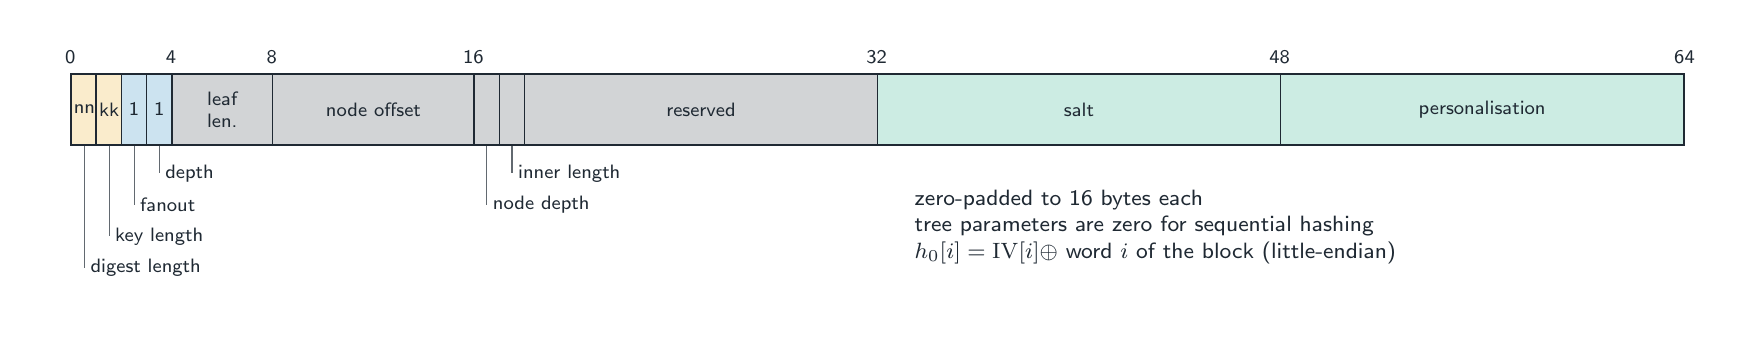
\begin{tikzpicture}[f/.style={draw=hsink, line width=0.6pt, minimum height=9mm, inner sep=1pt,
    font=\sffamily\scriptsize, align=center}]
  \def\u{0.16}
  % Field: start byte, length, label, colour.
  \foreach \s/\l/\lbl/\c in {0/1/{nn}/hsorange, 1/1/{kk}/hsorange, 2/1/{1}/hsblue,
      3/1/{1}/hsblue, 4/4/{leaf\\len.}/hsink, 8/8/{node offset}/hsink, 16/1/{}/hsink,
      17/1/{}/hsink, 18/14/{reserved}/hsink, 32/16/{salt}/hsgreen, 48/16/{personalisation}/hsgreen} {
    \node[f, fill=\c!20, minimum width=\l*\u*2 cm, anchor=west] (n\s) at (\s*\u*2, 0) {\lbl};
  }
  % Labels of the one-byte fields, staggered so that no leader line crosses a label.
  \foreach \s/\lbl/\k in {0/{digest length}/3, 1/{key length}/2, 2/fanout/1, 3/depth/0,
      16/{node depth}/1, 17/{inner length}/0} {
    \draw[hsink!70, line width=0.4pt] (n\s.south) -- ++(0,-0.35-0.4*\k)
      node[anchor=west, font=\sffamily\scriptsize, inner sep=2pt] {\lbl};
  }
  \foreach \s in {0,4,8,16,32,48} {
    \node[anchor=south, font=\sffamily\scriptsize] at (n\s.north west) {\s};
  }
  \node[anchor=south, font=\sffamily\scriptsize] at (n48.north east) {64};
  \node[anchor=north west, font=\sffamily\footnotesize, align=left] at (10.6,-0.9)
    {zero-padded to 16 bytes each\\
     tree parameters are zero for sequential hashing\\
     $h_0[i] = \mathrm{IV}[i] \oplus$ word $i$ of the block (little-endian)};
  \begin{scope}[on background layer]
    \coordinate (e1) at (-0.4,-2.4);
    \coordinate (e2) at (20.9,0.9);
    \node[card, fit=(e1)(e2), inner sep=4pt] {};
  \end{scope}
\end{tikzpicture}
\end{document}
